% sample.tex
\documentclass[20pt]{beamer}
\usetheme{default}
\beamertemplatenavigationsymbolsempty
\usepackage{listings}
\usepackage{multicol}

\definecolor{darkgreen}{rgb}{0,.5,0}

\lstset{language=Lisp,
  basicstyle=\ttfamily\scriptsize,
  stringstyle=\color{red},
  commentstyle=\color{darkgreen},
  breaklines = true,
}

\title[]{Dynamic C++}
\author[Jon]{https://github.com/
  JonChesterfield/
  dynamic\_cpp\_talk.git}

\begin{document}

\begin{frame}
  \titlepage
\end{frame}

\begin{frame}{Who are you listening to?}
  \begin{itemize}
  \item Software engineer
    \begin{itemize}
    \item C++ by income
    \item C by time spent
    \item Lisp by choice
    \end{itemize}
  \item Mostly writes
    \begin{itemize}
    \item Toolchains
    \item Datastructures
    \item Tests
    \end{itemize}
  \end{itemize}
\end{frame}

{
  \usebackgroundtemplate{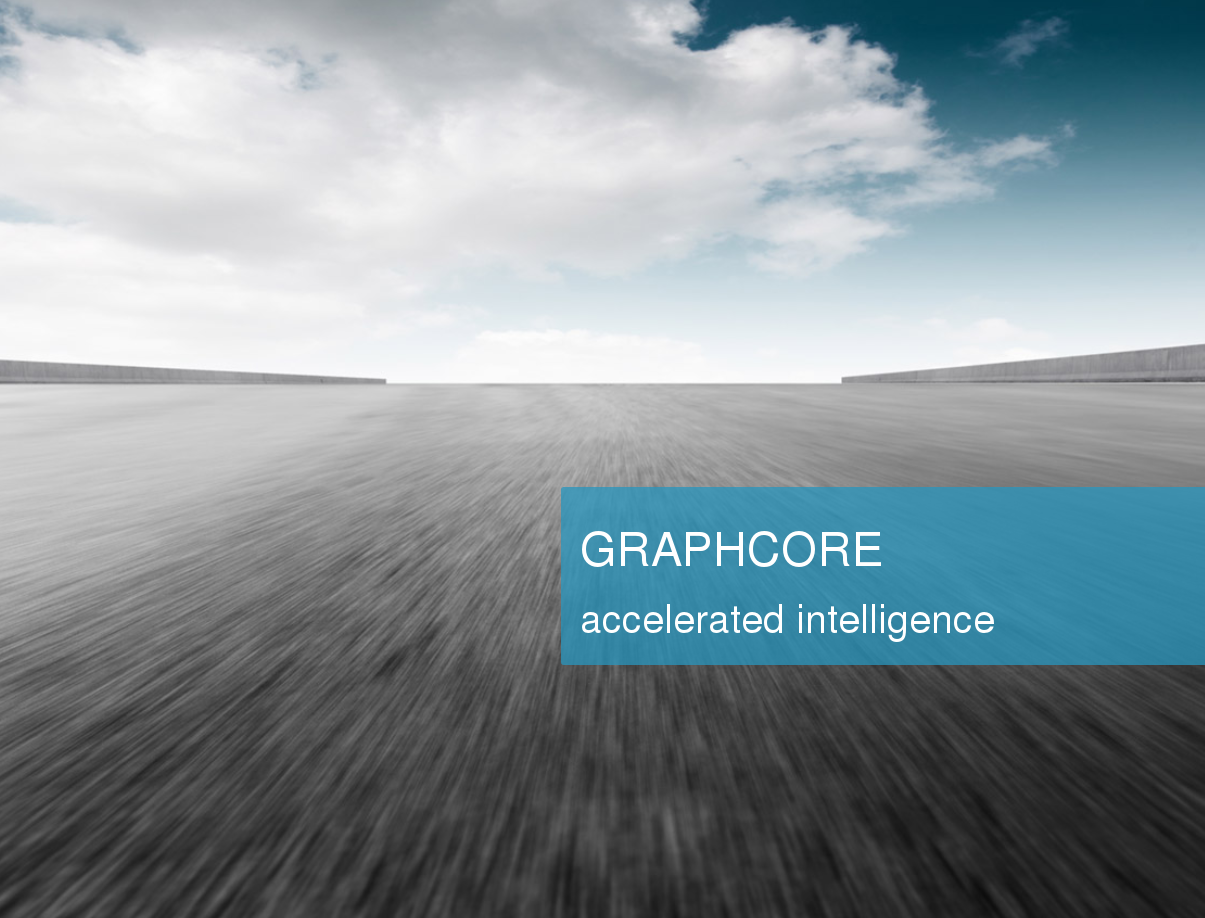
\includegraphics[width=\paperwidth]{graphcore-web.png}}
  \begin{frame}[plain]
  \end{frame}
}

\begin{frame}{Dynamic?}
  \begin{itemize}
  \item Dynamic typing
  \item Introspection
  \item Just in time
  \item Mutable metaclasses
  \item Object orientation
  \item eval-in-environment
  \item read-eval-print-loop
  \end{itemize}
\end{frame}

\begin{frame}{Static?}
  \begin{itemize}
  \item Static typing
  \item Template metaprogramming
  \item Compilation
  \item Immutable classes
  \item Class orientation?
  \item Embedded data
  \item Overnight builds
  \end{itemize}
\end{frame}



\begin{frame}{My background languages}
  \begin{multicols}{2}
    \begin{itemize}
    \item Assembly
    \item C
    \item C++
    \item Fortran
    \item Javascript
    \item Lisp
    \item Matlab
    \item Python
    \end{itemize}
  \end{multicols}
\end{frame}

\begin{frame}{Ease of use?}
  Because I want to get stuff done
  \begin{multicols}{2}
    \begin{enumerate}
    \item Javascript
    \item Matlab
    \item Python
    \item Fortran
    \item C
    \item C++
    \item Lisp
    \item Assembly
    \end{enumerate}
  \end{multicols}
\end{frame}

\begin{frame}{Flexibility?}
  Because I want to do difficult stuff
  \begin{multicols}{2}
    \begin{enumerate}
    \item Assembly
    \item Lisp
    \item Javascript
    \item Python
    \item C++
    \item C
    \item Matlab
    \item Fortran
    \end{enumerate}
  \end{multicols}
\end{frame}

\begin{frame}{Correlation?}
  \begin{columns}
    \column{0.5\linewidth}
    \begin{enumerate}
    \item Javascript
    \item Matlab
    \item Python
    \item Fortran
    \item C
    \item C++
    \item Lisp
    \item Assembly
    \end{enumerate}
    \column{0.5\linewidth}
    \begin{enumerate}
    \item Assembly
    \item Lisp
    \item Javascript
    \item Python
    \item C++
    \item C
    \item Matlab
    \item Fortran
    \end{enumerate}
  \end{columns}
\end{frame}

\begin{frame}{Expected performance?}
  In my experience. YMMV!
  \begin{multicols}{2}
    \begin{enumerate}
    \item Fortran
    \item C++
    \item C
    \item Matlab
    \item Python
    \item Javascript
    \item Lisp
    \item Assembly
    \end{enumerate}
  \end{multicols}
\end{frame}


\begin{frame}{Great parts of C++}
\end{frame}

\begin{frame}{Great parts of C++}
  \begin{multicols}{2}
    \begin{itemize}
    \item STL
    \item atomics
    \item auto
    \item catch
    \item exceptions
    \item llvm
    \item malloc
    \item performance
    \item preprocessor
    \item raii
    \item templates
    \item valgrind
    \end{itemize}
  \end{multicols}
\end{frame}

\begin{frame}{Terrible parts of C++}
\end{frame}

\begin{frame}{Terrible parts of C++}
  \begin{multicols}{2}
    \begin{itemize}
    \item aliasing
    \item classes
    \item compilation
    \item complexity
    \item inconsistency
    \item introspection
    \item macros
    \item parsing
    \item redundancy
    \item scoping
    \item the abi
    \item types
    \end{itemize}
  \end{multicols}
\end{frame}

\begin{frame}{Easy fixes}
  \begin{itemize}
  \item -fno-strict-aliasing
  \end{itemize}
\end{frame}

\begin{frame}{C++ static typing example}
  Persistent hashed trie.
  \begin{itemize}
  \item Represent varint pascal string
  \item Wanted a uint6\_t
  \item Typesafe conversions to uint8\_t
  \item Implicit type conversions
  \item Cannot represent contracts
  \end{itemize}
\end{frame}

\begin{frame}{Type systems in C++}
  \begin{itemize}
  \item Types on variables, not values
  \item Structural typing in templates
  \item Erasure(std::function, void *)
  \item Opaque types(char[], foo *)
  \item Nominal polymorphism dispatch
  \item Overloaded return type via proxy
  \item Non-transitive const \& mutable
  \end{itemize}
\end{frame}

\begin{frame}{Macros $|$ code generators}
  \begin{itemize}
  \item ln src/x.c gen/x.c
  \item python src/x.c.py $>$ gen/x.c
  \item clang -c gen/x.c -o obj/x.bc
  \end{itemize}

  \begin{center}
    \begin{tabular}{ |c|c|c| }
      \hline
      src & gen & obj \\
      \hline
      x.hpp & x.hpp & \\
      x.cpp & x.cpp & x.bc \\
      x.hpp.py & x.hpp & \\
      x.cpp.py & x.cpp & x.bc \\
      \hline
    \end{tabular}
  \end{center}
\end{frame}

{
  \usebackgroundtemplate{
\includegraphics[height=\paperheight]{DragonCrop.png}}
  \begin{frame}[plain]
  \end{frame}
}

\begin{frame}{How does LLVM help?}
  \begin{itemize}
  \item Clang gives C++ $=>$ bitcode
  \item lli is an interpreter for bitcode
  \item llvm-link is $x.bc + y.bc => z.bc$
  \item opt runs optimisation passes
    \begin{itemize}
    \item The built in ones
    \item Any you decide to write
    \end{itemize}
  \item llc gives bitcode $=>$ $x86\_64$
  \end{itemize}
\end{frame}

\begin{frame}{Tooling}
  \begin{itemize}
  \item clang
  \item rtags
  \item clang-format
  \item mcjit, orc jit
  \item domain specific optimisation
  \item various code sanitizers
  \item custom compilers
  \end{itemize}
\end{frame}

\begin{frame}{Compilation}
  \begin{itemize}
  \item Your library/program is a dir tree
  \item clang turns leaf .cpp into bc
  \item llvm-link turns directories into bc
  \item opt reduces the size of bc
    \begin{itemize}
    \item internalise symbols here
    \end{itemize}
  \item recurse...
  \item base case is one bc into library
  \end{itemize}
\end{frame}


\begin{frame}{Language bindings to C++}
  \begin{itemize}
  \item Parse C++ yourself? Use swig?
  \item Write the class api in .json?
    \begin{itemize}
    \item Generate the C++ header
    \item Generate the language bindings
    \end{itemize}
  \item Parse the bitcode instead
    \begin{itemize}
    \item Much friendlier than C++
    \item Parser already exists
    \item Maps directly to machine types
    \end{itemize}
  \end{itemize}
\end{frame}

\begin{frame}{C++ with Python}
  \begin{itemize}
  \item C++ can embed an interpreter
  \item Python can load a dyn library
  \item pybind11 makes the latter nicer
  \item 'iterators' similar enough
  \item refcounting + raii cooperate
  \item interactive testing via Python?
  \item writing hot loops in C++?
  \end{itemize}
\end{frame}

{
  \usebackgroundtemplate{
\includegraphics[width=\paperwidth]{The_GIMP_icon.png}}
  \begin{frame}[plain]
  \end{frame}
}

\begin{frame}{The GIMP}
  \begin{itemize}
  \item Core implemented in C
  \item Plugins can be written in
    \begin{itemize}
    \item C $|$ C++
    \item Scheme
    \item Python
    \item Perl
    \end{itemize}
  \item Core provides a set of types
  \item Each plugin provides functions
  \item Any plugin can call any function
  \end{itemize}
\end{frame}

{
  \usebackgroundtemplate{
    \vbox to \paperheight{
      \vfil\hbox to \paperwidth{
        \hfil
\includegraphics[height=\paperheight]{EmacsIcon.png}
        \hfil}
      \vfil}
  }
  \begin{frame}[plain]
  \end{frame}
}

\begin{frame}{Emacs, circa 1980}
  \begin{itemize}
  \item Core implemented in (nasty) C
  \item Mostly written in lisp
  \item Dynamically typed
  \item Dynamically scoped!
  \item Extensible at runtime
  \item Ridiculously large codebase
  \item (Somehow) still runs correctly
  \end{itemize}
\end{frame}

\begin{frame}{Your C++ IDE should...}
  \begin{itemize}
  \item Jump to definition
  \item Show all call sites
  \item Highlight syntactic errors
  \item Compile \& test on single key
  \item Automate source formatting
  \item Interop with source control
  \item Provide macros
  \end{itemize}
\end{frame}

\begin{frame}
  \titlepage
\end{frame}

\end{document}
